
\documentclass[bsc,frontabs,twoside,singlespacing,parskip,deptreport]{infthesis}
\usepackage{eurosym}
\usepackage{graphicx}
\usepackage{hyperref}
\hypersetup{unicode=true,
			colorlinks=true,
			linkcolor=black,
			urlcolor=cyan,
            pdfborder={0 0 0},
            breaklinks=true}
\urlstyle{same}
\providecommand{\tightlist}{%
  \setlength{\itemsep}{0pt}\setlength{\parskip}{0pt}}

\begin{document}

\title{RegEx Search \& Replace Extension for Chrome and Firefox}

\author{Dalimil Hajek}

\course{Computer Science}
\project{BSc Hons Project Report}
\date{\today}

\abstract{
The aim of this project was to build a browser extension that allows users to search and replace text with regular expressions in editable text input fields of web pages.

After evaluating existing extensions that were unsuccessfully attempting to implement this functionality, the new extension has been carefully designed, developed, and finally successfully released for Chrome\footnote{\url{https://chrome.google.com/webstore/detail/find-replace-for-text-edi/jajhdmnpiocpbpnlpejbgmpijgmoknnl}} and Firefox\footnote{\url{https://addons.mozilla.org/en-GB/firefox/addon/find-replace-for-text-editing/}} browsers.

In addition to the future-rich search and replace function, this plugin also adds the ability to save favorite patterns, store search history, or predefine text templates that can be inserted into the editable area of a page.

The software followed an iterative development process, where user feedback was collected via several means, including Google Analytics, which was used to track user interaction, and a support website used to collect user feedback comments.

After the initial release, about twenty updates have been subsequently released over the span of a few months. This iteration was further supported by automated tests of several kinds.

The extension has received excellent reviews, has been mentioned in a Medium article, and at the time of writing is installed on over 6000 devices (users from both browsers combined).
}

\maketitle

\section*{Acknowledgements}
Thanks to
\begin{itemize}
\item
  Boris Grot -- for supervising the whole project, and making important feature suggestions leading up to the first official releases of the extension on the Chrome and Firefox web stores
\item
  Michael O'Boyle -- for making suggestions, especially regarding Google Analytics
\item
  Christoph Metze -- for finding several important bugs that subsequently led to releases \texttt{1.3.2}, \texttt{1.3.3}, and \texttt{1.3.4}
\item
  Daniel Tomberlin -- for pointing out a use case when trying to search across multiple single-line inputs, and for updating his web store rating and review after I implemented it in \texttt{1.3.6}
\item
  GitHub user \href{https://github.com/MarkRH}{MarkRH} -- for finding a bug that was later fixed in \texttt{1.1.3}
\item
  StackOverflow user \href{https://stackoverflow.com/users/3959875/woxxom}{wOxxOm} -- for suggesting \texttt{Document.execCommand} API that I used to fix issues with templates in \texttt{1.2.0}
\end{itemize}

And also thanks to all those people who submitted user feedback or
reviews, and people who participated in the user study.

\standarddeclaration

\tableofcontents
\listoffigures

\chapter{Introduction} % should be about 5 pages
Modern web browsers allow users to find text in a web page, but when it comes to editable text areas that are often used on blogging platforms, online forums, social media, and email web clients, as a form of user input, none of the existing browsers allow users to also replace the found occurrences.
 
The aim of this project was to build an extension that adds this browser functionality. The tool allows users to find and replace text in editable text input fields of web pages, and includes a large set of features and search options, including regular expression support and occurrence highlighting.

\section{Motivation}
Search and replace functionality can be extremely useful when composing long emails, writing posts on social media, online forums, or blogging platforms, as well as in any email web clients. 

The most frequent use cases are:
\begin{itemize}
\item Fixing a typographical error -- A word or a phrase may have been used several times with the wrong spelling. This can occur several times in a forum post or an email, and it would be convenient to replace everything at once.

This also includes fixing unreadable characters in blog entries such as {\it \^{A}\euro\r{?}}, due to a change in encoding or some unintended text handling.

\item Normalizing incorrectly formatted text -- Regular expressions can be used to detect formatting errors such as multiple spaces before a period, missing upper-case letter, various metric unit formatting errors, and similar. Search and replace extension supporting regular expressions can quickly find and fix these.

\item Renaming a phrase -- Often a word or a phrase that occurs several times throughout a text needs to be corrected or substituted (perhaps using a synonym or a wording that sounds better)
\end{itemize}

Without having a browser extension for search and replace, one could imagine a solution where all text is copied and pasted into an advanced text editor, fixed using the built-in search and replace function, and copied back into the web page input field.

In addition to being a lengthy and time consuming process, this method would in many cases lose all text formatting, because more advanced editable text elements on the web may contain images, emojis, and text containing many formatting tags, which would not be preserved during the copy-pasting.

Additional motivation behind the development of this project was to add search-and-replace related features that are missing even from the more advanced text editors. One of them is storing the search history, and also being able to save favorite search patterns, that can later be quickly accessed. Both of these would save time and increase user's productivity.

\section{Existing Extensions}
Web browsers support standard search functionality for any text on a page but no browsers have the find \& replace functionality. Users have asked for this feature on Google Chrome forums\footnote{Google Chrome Forum link: \href{https://productforums.google.com/forum/\#!topic/chrome/Y4UORlpdYfo}{https://productforums.google.com/forum/\#!topic/chrome/Y4UORlpdYfo}}, but the decision of browser developers was to leave the implementation of this functionality to potential text-processing web applications, rather than implementing it as a part of the browser.

\begin{figure}[h]
\centering
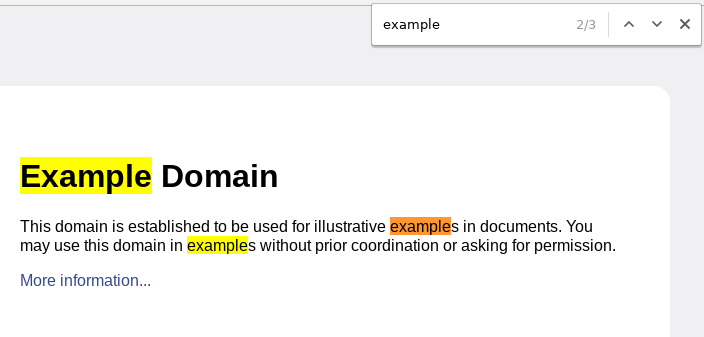
\includegraphics[width=0.6\textwidth]{../docs/browser-find-toolbar/chrome-find.png}
\caption{Google Chrome browser find tool}
\end{figure}

\begin{figure}[h]
\centering
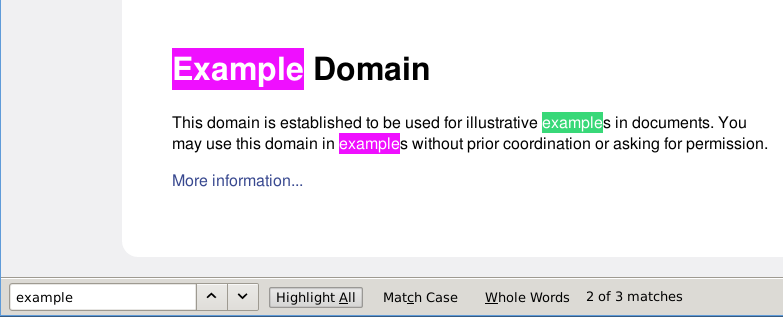
\includegraphics[width=0.6\textwidth]{../docs/browser-find-toolbar/firefox-find.png}
\caption{Mozilla Firefox browser find tool}
\end{figure}

There have been several attempts to implement this functionality via an extension. Most of them either don't work, are missing functionality (particularly support for regular expressions), are limited to certain websites, or are counter-intuitive and hard to use in general. 

\subsection{Chrome}

\begin{itemize}
\item
  {\bf Search and Replace}\footnote{\href{https://chrome.google.com/webstore/detail/search-and-replace/bldchfkhmnkoimaciljpilanilmbnofo}{https://chrome.google.com/webstore/detail/search-and-replace/bldchfkhmnkoimaciljpilanilmbnofo}}
  
  \begin{itemize}
  \tightlist
\item
  This is the dominant one with over 52,000 downloads (as of Mar 2018)
\item
  It has only $3.1/5$ stars and many reviews are complaining it doesn't work or that it destroys other content of the current page
\item
  It has usability issues (control UI is partially hidden) and it doesn't work in many places such as Blogger or Facebook
\item
  This is a very bad and simplistic solution that is mostly broken but benefits from a larger user base because it appeared in the web store in 2013
  \end{itemize}
  
\item
  {\bf Find Replace}\footnote{\href{https://chrome.google.com/webstore/detail/find-replace/cfjmfciolkikfodjfdmdpdmpfbjdofek}{https://chrome.google.com/webstore/detail/find-replace/cfjmfciolkikfodjfdmdpdmpfbjdofek}}
  \begin{itemize}
  \tightlist
\item
  This extension requires copy-pasting your desired text into the provided box (it is plain-text only, so formatting is lost).
\item
  It has almost 1000 users (as of Dec 2017), but it has been around since 2013
\item
  It is unable to perform the search and replace in browser. This is no better than copy pasting text into a text editor and performing the operation there
  \end{itemize}
\item
  \textbf{FindR}\footnote{\href{https://chrome.google.com/webstore/detail/findr/bidnaaogcagbdidehabnjfedabckhdgc}{https://chrome.google.com/webstore/detail/findr/bidnaaogcagbdidehabnjfedabckhdgc}}
  \begin{itemize}
  \tightlist
\item
  It has around 2000 users and $3.8/5$ stars. It has been in the web store since April 2016.
\item
  This extension is used for replacing any HTML text in the page, rather than text in input fields -- for this purpose it seems to work, but when one tries to use it only for text input fields, things break and the extension stops working (highlighting and match indicator both disappear and replace button stops working)
\item
  It also requires permission to \textit{Read and change all your data on the websites that you visit}, which might be a privacy issue (the extension can read everything even when the user is not using it)
  \end{itemize}
\item
  \textbf{Easy Replace}\footnote{\href{https://chrome.google.com/webstore/detail/easy-replace/ojoeejfegihohnkjlfoonbnailkohkce}{https://chrome.google.com/webstore/detail/easy-replace/ojoeejfegihohnkjlfoonbnailkohkce}}
  \begin{itemize}
  \tightlist
\item
  It has over 3000 users but only $2.6/5$ stars
\item
  Most of them report it doesn't work because it only focuses on plain-text text areas and completely ignores more advanced editable HTML elements that most sites use these days
  \end{itemize}
\end{itemize}

\subsection{Firefox}

\begin{itemize}
\item
  \textbf{Find and Replace for Firefox}\footnote{\href{https://addons.mozilla.org/en-US/firefox/addon/find-and-replace-for-firefox}{https://addons.mozilla.org/en-US/firefox/addon/find-and-replace-for-firefox}}
  \begin{itemize}
  \tightlist
\item
  Old add-on, not compatible with the latest Firefox 57.
\item
  It has over 2000 users but only $3.4/5$ stars
\item
  It's not working for most users, has almost no options (no RegEx, no highlighting, etc.)
\item
  It was last updated in 2012 and is not maintained
  \end{itemize}
\item
  \textbf{FoxReplace}\footnote{\href{https://addons.mozilla.org/en-US/firefox/addon/foxreplace/}{https://addons.mozilla.org/en-US/firefox/addon/foxreplace/}}
  \begin{itemize}
  \tightlist
\item
  This extension provides different functionality -- it asks the user to initially define a list of substitutions and then it automatically applies them globally across the text in newly loaded web pages
\item
  FoxReplace has over 7000 users (Mar 2018) but targets a different audience
  \end{itemize}
\end{itemize}

\subsection{Other Browsers}
Supporting more browsers adds extra work, so it would only make sense if these browsers represent a significant portion of the market. The usage share of browsers is measured by various methods and is often quite inaccurate (see \cite{W1}). \\
Approximate values for usage share for desktop browsers in Dec 2017 are (taken from \cite{A1}): Chrome 65\%, Firefox 12\%, IE 8\%, Safari 6\%, Edge 4\%.

This project focused on Chrome and Firefox, which together represent a large portion of the overall market, and which both mostly follow the same Extension API (there are only a few differences \cite{M5} so we didn't need to have separate code-bases).

Safari, although widely used by Mac users, has its own extension API and is in general much more involved as it requires dealing with Apple's developer libraries and licenses, so we decided not to develop an extension for this browser.


%The Introduction chapter should always provide a 'roadmap' to the report. Of course it should provide an introduction to the problem being considered, but it should also give some details of what you did -- do not leave this to the conclusion. You should give forward references into the rest of the report -- e.g., "In Chapter 2 how algorithms and heuristics are used to deal with approximate counting are discussed", "The design of the system is presented in Chapter 4", "In Chapter 3 the reasons for choosing to focus on the bounded-degree case of this problem are explained". 

% make sure you point out what was involved in solving certain problems; this can help a non-expert judge the work involved. For instance: "The interpolation algorithm was implemented in C directly, rather than using the routines in Matlab". "In order to develop a user interface appropriate for the educational system, 4 prototypes were tested on 50 students". 

% Use passive voice: A and B were used. instead of I used A and B


\chapter{Background}
A browser extension is a bundled collection of files -- HTML, CSS, JavaScript, images and other assets, that together add functionality to the browser. They have access to the standard DOM API (same as a regular website) but in addition to that they can access the WebExtensions API, which is provided by the browser. At the time of writing, the WebExtensions API is to a large extent (only with slight deviations in implementations) supported by Mozilla Firefox, Google Chrome, Microsoft Edge, and Opera browsers (see detailed explanation in \cite{C1}, \cite{C2}, \cite{M6} and \cite{M7}).

A typical extension consists of a background page, which holds the main logic of the extension and has full access to the APIs, pop-up widget, which presents the extension's user interface, and one or more content scripts, which are pieces of JavaScript code that are injected into the current web page so that we can interact with its content.

After installing a browser extension in Chrome or Firefox, a small icon representing the extension is added to the top toolbar. When users click this icon, the extension displays its pop-up widget. The standard way to present an interface to the user is via this widget. One could come up with alternative ways to present extension's UI but this design pattern using a pop-up is the preferred way and something that users expect by default. Since a pop-up widget works well in our scenario, we decided to proceed with that.

\chapter{Design}

\section{Naming and Search Engine Optimization}
Based on the competition research mentioned in the introduction chapter above, the following extension names already existed: \textit{Easy Replace}, \textit{Search and Replace}, \textit{FindR}, \textit{Find Replace}, \textit{FoxReplace}. Using any of these existing names would be bad for the SEO and discoverability, and would most likely lead to confusions.

At the same time, we wanted to clearly indicate that the extension is used for input fields and editable content rather than HTML source code.

People are likely to search for browser extensions by typing in the functionality that they need. In our case, that might look something like "find and replace in text input fields extension". We predicted that stating the extension's purpose in its title and description could help us do better in search results. Therefore, we avoided any newly-invented words and named it \textit{Find \& Replace for Text Editing}. We are not trying to trademark a new brand name, we are simply trying to match what people might search for, so that is why this name was chosen.

The naming idea was largely successful. In March 2018 (a few months after the first release), the extension ranked 2nd in the Google search results for queries \textit{search and replace in firefox}, and \textit{search and replace browser}, and ranked 1st for the queries \textit{search and replace in chrome}, and \textit{find and replace in browser}.\footnote{Tested using incognito modes in both Firefox and Chrome, and searching via www.google.co.uk on 15th March 2018}

At the time of writing, organic Google Search remains to be the primary user acquisition source. Almost 80\% of all downloads of the extension in the Chrome Web Store are users who came there from Google Search results. This evaluation is further discussed in \autoref{chapter:evaluation}.

\begin{figure}[h]
\centering
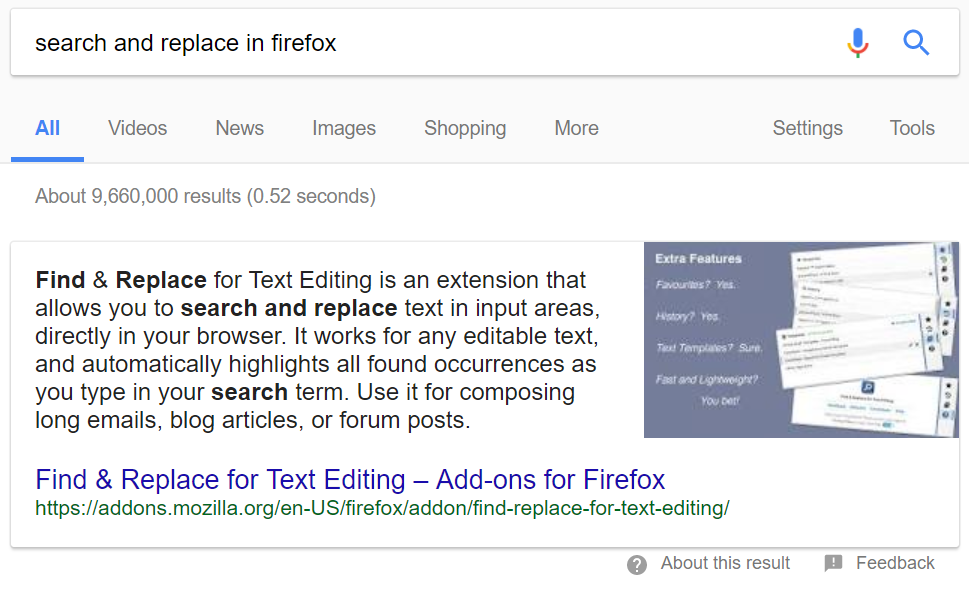
\includegraphics[width=0.7\textwidth]{../docs/search-results.png}
\caption{Google Search Results Ranking}
\end{figure}

\section{User Interface Inspiration}
To some extent, we wanted to follow the current standard of find \& replace toolbars. Many of these can be seen in more advanced text editors. The user interfaces of some of the popular ones were examined and used as an inspiration.

\begin{figure}[hp]
\centering
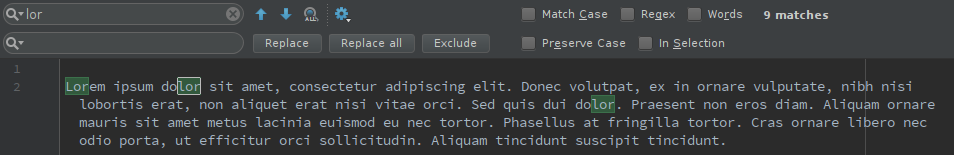
\includegraphics[width=0.9\textwidth]{../docs/editor-find-and-replace/android-studio-find-and-replace.png}
\caption{Android Studio find and replace tool}
\end{figure}

\begin{figure}[hp]
\centering
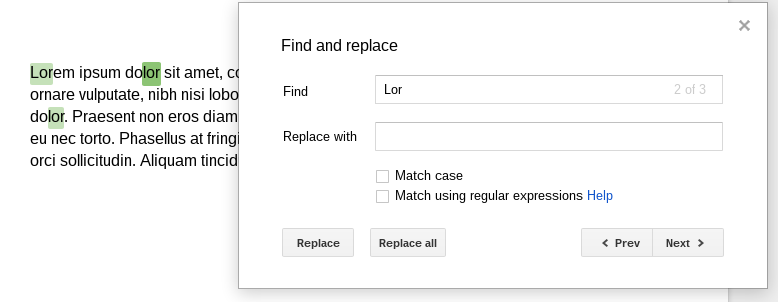
\includegraphics[width=0.9\textwidth]{../docs/editor-find-and-replace/gdocs-find-and-replace.png}
\caption{Google Docs find and replace tool}
\end{figure}

\begin{figure}[hp]
\centering
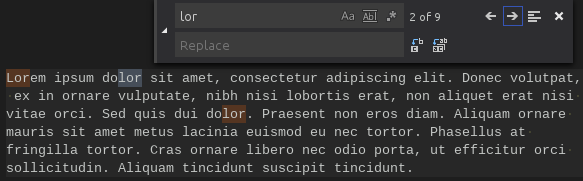
\includegraphics[width=0.9\textwidth]{../docs/editor-find-and-replace/vscode-find-and-replace.png}
\caption{Visual Studio Code find and replace tool}
\end{figure}

\begin{figure}[hp]
\centering
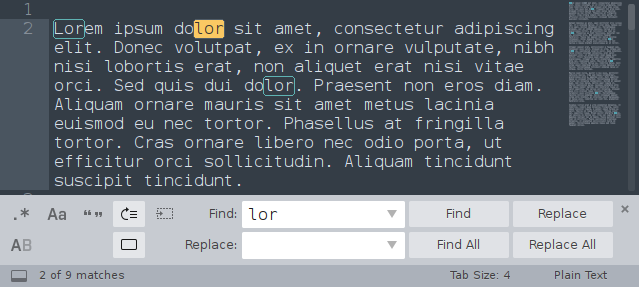
\includegraphics[width=0.9\textwidth]{../docs/editor-find-and-replace/sublime-find-and-replace.png}
\caption{Sublime Text 3 find and replace tool}
\end{figure}

We wanted our extension to follow some of the design patterns that the existing text editors use, so that users are presented with a user interface that they can easily understand and start using quickly.

At the same time, it should not be assumed that average users are familiar with regular expression or more advanced search functions. Therefore, the UI design of some of these editor widgets should only be used as an inspiration -- average users are not developers and the number of options in this extension must not feel overwhelming.

\section{UI Components}
To support all the functionality that we specified, the extension widget should have the following UI elements:
\begin{itemize}
\tightlist
\item
  \textit{Find} input field
\item
  \textit{Replace} input field
\item
  \textbf{Action buttons}

  \begin{itemize}
  \tightlist
  \item
    Replace
  \item
    Replace All
  \item
    Find next
  \item
    Find previous
  \item
    Save to favorites
  \item
  	Expand/Collapse advanced search options
  \end{itemize}
\item
  \textbf{Options}

  \begin{itemize}
  \tightlist
  \item
    Match Case (Aa)
  \item
    Whole Word (Ab\textbar{})
  \item
    Use Regex (.*)
  \item
    Limit to Text Selection
  \end{itemize}
\item
  \textit{X of Y} or \textit{No Results} indicator
\item
  Regex groups indicator (for regex search only)
\item
  \textbf{Panel tabs}

  \begin{itemize}
  \item
    Favorites
  \item
    History
  \item
    Templates
  \item
    Help/Info/Feedback
  \end{itemize}
\end{itemize}

We split the user interface layout into two types -- simple and advanced. Because displaying all search options in one widget might feel overwhelming for average users, there is a way of switching the search UI to the \textit{advanced} state that includes regex options and helpful previews of matched regex groups etc.

\begin{figure}[h]
\centering
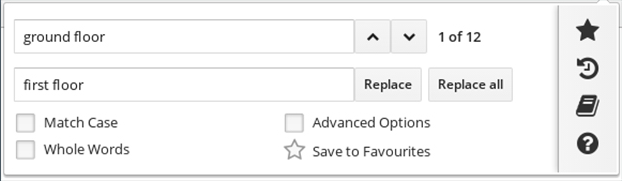
\includegraphics[width=0.95\textwidth]{../graphics/search-widget-simple.png}
\caption{Search widget UI -- simple view}
\end{figure}

\begin{figure}[h]
\centering
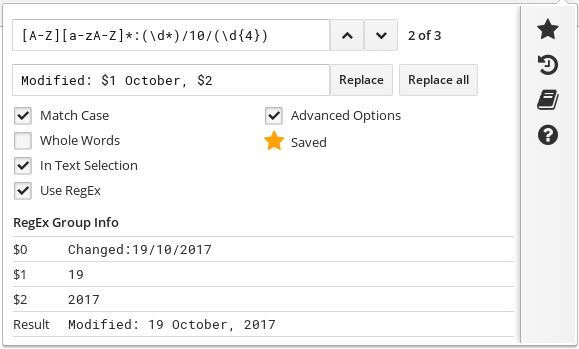
\includegraphics[width=0.95\textwidth]{../graphics/search-widget-advanced.png}
\caption{Search widget UI -- advanced view}
\end{figure}

\section{Why not Material Design}
For the general look and feel, it was decided not to use Google's increasingly popular Material Design \cite{A2} for several reasons. First, Material Design works well when there is a lot of space and all the elements can be spread out. Unfortunately, this extension's user interface is a small widget with very limited space and many condensed components.

Secondly, Material Design likes to add its \textit{ripple effect} to most interactions (such as clicking a button). This looks great for actions that have large impact (e.g. navigating to a new page, or submitting a form), but for our purposes we need something less flashy, as most buttons are going to be pressed very often (\textit{Find next} and \textit{Replace} buttons) and too many effects or animations would present too much distraction for the user.

An extension (a pop-up widget) like ours should, to a large extent, feel like it is part of the browser by perhaps matching some of the user interface styles. We don't want to create an extension that gives users the feeling that it completely doesn't belong because of its wild user interface and flashy styles.

\section{Scope of Search}
Instead of searching in any visible text or simply the HTML source code, we want to limit our search only to elements that contain editable text. There are several ways to create an editable area on web. These are described in \cite{M1} and \cite{P1}.

\subsection{\texttt{\textless{}input\ type="text"\textgreater{}}}

For a short single line of text, HTML
\texttt{\textless{}input\textgreater{}} element is often used. There are
other types of input fields (many new were added with HTML5), such as
date, email, number, tel, time, and similar, but text is the standard
one (see \cite{M2}).

However, due to the short length (20 characters by default), this is not the kind of input that needs the find \& replace functionality on its own. The primary use case of our extension are large multi-line text areas, but we also include the short single-line input kind to allow users to search and replace text in a page across many single-line inputs simultaneously.

\subsection{\texttt{\textless{}textarea\textgreater{}\textless{}/textarea\textgreater{}}}

Multi-line plain-text input space (see \cite{M3}). This should be a common target for find \& replace. It is used by many sites to allow users compose longer pieces of text, one of them is a new post creation process on Reddit.

\subsection{\texttt{\textless{}div\ contenteditable="true"\textgreater{}\textless{}/div\textgreater{}}}

Enabling rich text formatting by allowing HTML tags inside the text
area, \texttt{contenteditable} elements are used in Gmail, Facebook
posts, Facebook Messenger, GitHub editor, Twitter, and many other sites.

Note that \texttt{contenteditable} is a global attribute and is
therefore not limited to \texttt{div} tags (see \cite{M4}).

\subsection{\texttt{contenteditable} tag inside 
\texttt{\textless{}iframe\textgreater{}\textless{}/iframe\textgreater{}}}

Blogger.com is an example of a site that isolates the main
contenteditable area in an iframe. When performing find \& replace we
must consider the scenario where we are dealing with elements inside an \texttt{\textless{}iframe\textgreater{}} on the page.

\subsection{Other DOM}
This extension is not meant to modify (find \& replace) the raw HTML text of the page's source. It is limited to finding occurrences in text areas that are modifiable by users.  

There are certainly sites that might try to avoid all the options discussed above and implement their own text editor functionality. One notable example is Google Docs, which is using static DOM but listen to user's keyboard events to modify it internally in JavaScript. Implementing an online text editor from scratch without using contenteditable or textareas involves a lot of programming work, and such editor should probably include its own find \& replace functionality anyway, which is exactly what Google Docs do.

At the time when the project was first designed, it seemed reasonable to exclude single-line inputs from the scope, as their small editable input space didn't seem suitable for our search and replace functionality. After receiving a lot of user feedback which revealed new use cases, single-line inputs were included in the search scope via an optional checkbox option in the search widget (to ensure backward compatibility and no unexpected behavior for existing users).

\chapter{Implementation}

\section{Component Overview}
As mentioned before, our extension consists of three main components -- a pop-up widget presenting the search UI to the user, a few content scripts, which are pieces of JavaScript code that are injected into the current web page so that we can interact with its content (e.g. perform the search and highlighting), and finally an invisible background page, which has full access to the privileged extension APIs (other extension components do not) and performs our content script injection whenever the user launches the extension's search widget.

We designed our extension with privacy in mind, so that is why instead of giving the extension permission to access all browser tabs and being able to automatically run, it can only start operating in the current tab once the user launched the search widget, not before. This involved more work, as we had to implement the dynamic content script injection, set up the relevant event listeners, and add addition logic to prevent repeated script injection after switching between browser tabs back and forth.

Despite having to write significantly more code, it allowed us to get rid of the extra permissions we would otherwise need to request in the extension manifest. These permissions are displayed to the user just before installation and requesting one that can \textit{Read and change all your data on the websites that you visit} is definitely one that we wanted to avoid, as it could discourage many users. This way we do not need any special permissions.

\subsection{Component Life-cycle}
Our background page is only a single JavaScript file that sets up all required events and starts listening to incoming message connections. Whenever the extension icon is clicked (or the launch keyboard shortcut pressed), our UI widget pops up. The widget can be closed by the user anytime, so it first registers itself with our background page, so that the background page can see when the message port disconnects (signaling that the widget was closed). 

The widget needs to communicate with the content script to manage the search and highlighting in the page. Right after the widget connects to the background page, the background page checks if the content scripts have been injected already (the widget may have been previously closed and reopened). If they have not been injected yet, it injects them. If, on the other hand, they have been previously injected, it simply sends a message to the content script to reconnect (restart its port connection). 

Once our main content scripts are injected, they broadcast a port connection -- both the background page and UI widget are listening for this event. The background page needs to connect to the content script to see when the message port disconnects (user may have navigated to a different page and we thus lost the injected code). Search widget needs the content script connection for all its API actions -- this is our main message passing channel.

The life-cycle of our extension is complicated because we are managing three separate component -- the search widget, the background page, and the context of the webpage itself (via content scripts). None of these components are permanent. The search widget can be destroyed anytime, the content scripts in the page are lost whenever the user navigates to a different website, and finally the background page is not persistent either -- it simply sets up a collection of event listeners and waits for the browser to wake it up (see \cite{C6}).

\section{Search Widget}
To implement the search UI widget, we could simply create DOM elements for all the input components and listen to any changes as the user interacts with the UI. Unfortunately, all input components manage their own state -- a better approach would be to store the state of the search parameters in one central place/datastore and have the UI inputs reflect this data. Therefore, we used the React.js library to implement the user interface.

The React library \cite{A3} has become very popular in recent years -- one reason is that it enforces the pattern of always reflecting the current application state in the UI. React's internal state is the single source of truth (see React input handling \cite{A4}).

Without it, we would have to manage all the inputs separately and this could create many UI inconsistencies -- incorrect update of our internal data might create a state of the application where our search parameters are set to certain values internally but display different state externally via our UI. As we are dealing with a lot of different inputs (many search parameters as well as the simple and advanced modes of the search layout), using React seemed to be a wise choice.

Note that React is only a JavaScript library that allows for a particular way of implementing UI code, but itself doesn't provide any predefined components or styling. The search widget UI was built from scratch without using any existing stylesheets or components.

We set up the project so that we can test the UI widget components in isolation, without creating an actual browser extension and calling the relevant APIs. During development we simply mount our root UI component on a regular website. In production, the same component is mounted in the place of the pop-up widget, which also behaves as a web page.

To also support React's JSX syntax (see \cite{A5}) and the newest ECMAScript language standards, we used Babel \cite{A6} for compiling our JavaScript sources. We used Webpack \cite{A7} to bundle all our source code into a single file, which is obfuscated and small in size. Both of these libraries are widely used and often used in conjunction with React.

\section{User Actions API and Message Passing}
Whenever user performs an action such as clicking the button \textit{Replace} or typing something into the \textit{Find} input field, we send a message from the search widget to our content script running in the context of the page. We defined our custom API to specify what kind of messages can be exchanged and in particular what their payload should be.

This was needed because the user receives information from the extension in two ways - either via visual feedback from the content script running in the web page (match highlighting) or via the widget pop-up (search interface). These two components are separate and can only communicate via the messaging API \cite{C5}.

First we specified actions that users can perform using the search widget that also need to communicate with the page. The actions are the following. Note that actions that are local to the search widget and do not need to communicate with the page (such as tab navigation in the search widget) are intentionally omitted.

\begin{itemize}
\tightlist
\item
  Update search query or search options
  \begin{itemize}
  \tightlist
  \item
    Change the content of the \textit{Find} input field
  \item
    Toggle one of the search option checkboxes
  \end{itemize}
\item
  Find next/previous
\item
  Replace current/all
\item
  Insert a template
\item
  Close the widget
\end{itemize}

User actions specified above directly translate to types of messages
that need to be passed between our widget and the content scripts in the page. We define the following API, where each message has the prototype \texttt{\{action:\ string,\ data:\ Object\}} where \texttt{data} is for certain types of messages omitted:

\begin{itemize}
\tightlist

\item\textbf{action: updateSearch}

\begin{itemize}
\tightlist
\item
  Uses the \texttt{data} object to obtain matching search results
\item
  Response object:
  \texttt{\{invalidRegex:\ boolean, invalidSelection:\ boolean,\\ searchIndex:\ number, searchCount:\ number, currentMatch:\ object\}}
\end{itemize}

\item\textbf{action: findNext}

\begin{itemize}
\tightlist
\item
  Finds the next match
\item
  Returns:
  \texttt{\{searchIndex:\ number, searchCount:\ number,\ currentMatch:\ object\}}
\end{itemize}

\item\textbf{action: findPrev}

\begin{itemize}
\tightlist
\item
  Finds the previous match
\item
  Response identical to the \textit{findNext} action
\end{itemize}

\item\textbf{action: replaceCurrent}

\begin{itemize}
\tightlist
\item
  Replaces the current match with \texttt{data} contents
\item
  Response identical to the \textit{findNext} action
\end{itemize}

\item\textbf{action: replaceAll}

\begin{itemize}
\tightlist
\item
  Replaces all matches with \texttt{data} contents
\item
  Response identical to the \textit{findNext} action
\end{itemize}

\item\textbf{action: insertTemplate}

\begin{itemize}
\tightlist
\item
  Inserts template text \texttt{data} at current cursor
\item
  Returns: \texttt{\{noCursorPosition:\ boolean\}}
\end{itemize}

\item\textbf{action: shutdown}

\begin{itemize}
\tightlist
\item
  Clean up all active highlights and reset search when widget is closed
\end{itemize}

\item\textbf{action: restart}

\begin{itemize}
\tightlist
\item
  Trigger port reconnect action, on widget re-open
\end{itemize}

\item\textbf{action: log}

\begin{itemize}
\tightlist
\item
  Logs \texttt{data} (we disable this in production environment) 
\end{itemize}
\end{itemize}

Object \texttt{currentMatch} that is often returned as a part of the response message is used to display advanced regex information about matched regex groups. It has the following structure:
\texttt{\{groups:\ Array\textless{}string\textgreater{},\ replace:\ string\}}

We set up our messaging API this way because we want to minimize the amount of data that need to be exchanged between the extension's search widget and the page. The content script receives a search request from the search widget, performs the search, highlights matches, and returns status information back to the search widget. 

The other API calls follow a similar pattern, where the content script is asked to perform a certain action in the web page and return new status information back to the search widget afterwards (i.e. the number of matches, the current match, etc.).

\section{Content Scripts}
\subsection{RegExp Search}
JavaScript contains native support for regular expressions (see \cite{M8}). Without using any additional libraries, we can simply create new RegExp objects and execute search methods on regular strings to find matches for the given regular expression query. As long as we limit our search to visible text in editable text areas (rather than raw HTML source), finding occurrences is not a problem. The real challenge comes with visually highlighting the found matches in the page. Ideally, we would like to match the behavior of modern text editors and show to the user all found matches at once using text highlighting.

\subsection{Highlighting}
\begin{figure}[h]
\centering
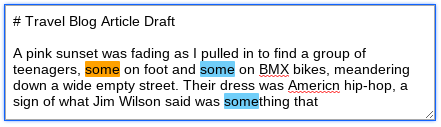
\includegraphics[width=0.7\textwidth]{../main/images/help/highlighting.png}
\caption{Match highlighting}
\end{figure}

\subsubsection{Highlighting in \texttt{contenteditable}}
We can highlight a piece of text inside a \texttt{contenteditable}
element by simply injecting our own \texttt{span} element with our
custom class into the element's DOM. Contenteditable elements are
designed to contain any HTML nodes so we are allowed to do this.

We ended up using the \textit{mark.js} \cite{A23} open-source plugin for the highlighting operation. We could certainly implement the highlighting ourselves (wrapping each search occurrence in \texttt{\textless{}span\textgreater{}} elements with custom styling),
but there are many tricky cases that we would need to handle. For
instance, HTML \texttt{\textless{}div\textgreater{}John\ \textless{}b\textgreater{}Smith\textless{}/b\textgreater{}\textless{}/div\textgreater{}} matches the query \texttt{John\ S} but simply inserting a \texttt{\textless{}span\textgreater{}} at the start and end would violate HTML rules, and instead we would need to create two pairs of \texttt{\textless{}span\textgreater{}} elements -- for \texttt{John} and another for \texttt{S} inside the \texttt{\textless{}b\textgreater{}} tags.

There are more tricky cases like this. Therefore, rather than
reinventing the wheel, it was wiser to use a plugin that is actively
maintained and can handle these cases for us.

\subsubsection{Highlighting in \texttt{\textless{}textarea\textgreater{}}}
Highlighting text in \texttt{\textless{}textarea\textgreater{}} was more tricky because this HTML element only allows plain text to be displayed inside it. Any styled markup will not render as expected. To overcome this, one must create an overlay with invisible text that exactly matches the textarea element and then highlight text in this new element. Further, there are many browser-specific quirks and one must also take care of synchronizing scrolling and handling textareas that are resizable by the user (the fact that it is a lot of work is discussed in \cite{A24}).

Fortunately, there have previously been a few attempts to implement this. The most successful version we found was a Will Boyd's jQuery plugin\footnote{\url{https://github.com/lonekorean/highlight-within-textarea/}}, because to some extent it also supported resizable textareas (other plugins we found did not).

Even though this plugin did better than all the other plugins, it still had many issues, particularly when it came to transferring all necessary CSS styles from the source textarea to the overlay element. During testing, it failed to properly align text for multiple textareas with various styling.

Therefore, we contributed to the development of this open-source plugin by fixing all the bugs we found and creating a pull-request on GitHub (with 10 new commits fixing various issues).\footnote{\url{https://github.com/lonekorean/highlight-within-textarea/pull/19}}

After two code reviews done by the author of the original plugin, this remains unmerged (at the time of writing). This is because the author had conflicting views on the design and purpose of the plugin (we are dynamically injecting the plugin code, which is a somewhat different use case) and he was also worried about backward-compatibility. 

We kept maintaining the updated forked version, which should hopefully help other people developing textarea highlighting. It has already been referred to in one other GitHub issue created by a different user.\footnote{\url{https://github.com/lonekorean/highlight-within-textarea/issues/21\#issuecomment-345318936}}

\subsubsection{Highlighting in \texttt{\textless{}input\textgreater{}}}
We initially excluded single-line input fields from the search as these are only very short pieces of text (typically only a few words), but after receiving user feedback it turned out that there are scenarios when there is a large number of single line text inputs in a single page and someone needs to search and replace a phrase across all of them at once.

The problem was that including single-line inputs by default could degrade the user experience because websites have plenty of search bars or input fields scattered around, often away from the main content. Therefore we added the choice to include single-line inputs in search as a switchable option.

Single-line input elements, similar to HTML textareas, only display plain-text, so for the highlighting we reused some of the code we already had for mirroring and overlaying textareas. The majority of changes were related to the overlay styling, because the input is vertically centered by default and instead of the text wrapping to the next line, it continues as a single line.

Handling the horizontal scroll was problematic however. Firefox correctly fires the scroll event that we were able capture to shift our overlay highlighting by the same scroll amount, but Chrome, on the other hand, does not fire the scroll event at all. It instead automatically resets the scroll position to zero after the element is defocused. So while the initial highlighting will always be correctly aligned, horizontally scrolling the input box with the search widget open will not move the highlights. Since single-line inputs with a large text overflow are quite uncommon in the first place, we ignore this specific case as it presents only a slight visual flaw that will most likely not occur.

\subsection{RegExp Replace}
To make regular expression search with matched groups useful, we allow the user to refer to matched subgroups in the \textit{Replace} input string via the following special symbols.

\begin{itemize}
\tightlist
\item
  \texttt{\$n}, where \textit{n} is a positive integer, inserts the n-th parenthesized submatch string.
\item
  \texttt{\$0} or \texttt{\$\&} both insert the full matched substring.
\end{itemize}

These patterns are commonly used to extend find \& replace functionality in advanced text editors. Inspiration to implement these symbols was also taken from Mozilla's spec on MDN website \cite{M9}.

We search for these symbols in the \textit{replace string}, and when the user clicks the \textit{Replace} button we substitute the appropriate subgroups (if they are found) for the current replacement in the page.

\subsection{Choosing Target Area Element}
By default the extension uses all available text areas in the page as the target of the search and replace operation. However, it is often the case that the user only wants to search in the text area that they are currently editing. We therefore implemented two modes of operation, either the user has no active area selected and the search is executed across all text areas in the page, or they place their active cursor in a specific text area, which is then chosen as the one and only target of the search operation.

To find the currently active element we used browser Document object's \texttt{activeElement} property (see \cite{M10}). This can be an \texttt{iframe} however, which is a different Document and Window context. So we had to first implement recursive search for our active element (iframes can be nested) to determine the correct Window and Document objects that should be used for all DOM operations (such as highlighting and finding matches in the page).

Identifying the right scope was also important for the cursor text selection, as one can have multiple text selections active at the same time (inside different simultaneously displayed iframes).

Even though nested iframes should not be too common in web page design, we had to handle the possibility to ensure correctness, rather than assume that there can only be at most one iframe at a time. We also created a test case to cover the nested iframes scenario.

\section{Accessibility}
Having read the Chrome extension accessibility guidelines \cite{C4}, we implemented several usability improvements that benefit not only people with disabilities but also regular users who can get things done more quickly or can more easily use the extension. 

\subsection{Keyboard}
We implemented keyboard shortcuts that can be used to control the extension more efficiently. One can launch the search widget with \texttt{Ctrl+Shift+F} (\texttt{Command+Shift+F} on
Mac). Note that all \texttt{Ctrl+F}, \texttt{Ctrl+R}, and
\texttt{Ctrl+Shift+R} were already predefined browser shortcuts, so we could not use those.

Once the search widget appears, the following operations can performed using the keyboard:
\begin{itemize}
\tightlist
\item
  Next match: Pressing \texttt{Enter} when focused in \emph{Find} input field
\item
  Previous match: Pressing \texttt{Shift+Enter} when focused in \emph{Find} input field
\item
  Replace: Pressing \texttt{Enter} when focused in \emph{Replace} input field
\item
  Replace All: Pressing \texttt{Shift+Enter} when focused in \emph{Replace} input field
\end{itemize}

\subsection{Browser Context Menu}
We added a new item to the browser's text-selection context menu. Users can select text on the page and, after right-clicking the selection, search for the text using the extension. This would ideally open the extension's search widget and substitute the selected text in the \textit{Find} input field. 

Unfortunately the extension API currently does not support opening the pop-up programmatically \cite{A19} -- the user must click the extension icon or press the keyboard shortcut to open it. Until the extension API is updated we can at least inject a script into the current page that creates a floating div notifying the user that they should press the keyboard shortcut to open the search widget. We can substitute the selected text in the \textit{Find} field in the background, so the users will immediately see the search results for their selected text once they open the widget.

\subsection{Search Widget Accessibility}
To improve the usability of our search widget, we initially disable the action buttons when the user hasn't typed in anything into the search field yet. This is in order to draw attention to the active input field element, rather than overwhelming the user with options that cannot be used (e.g. clicking \textit{Find next} when there is nothing to find). Google Docs use the exact same design pattern. 

To better indicate the target elements of our extension in the page, we add a box shadow highlight to the currently selected input area. If no single text area is selected, we highlight all text areas in the page (because the default is to search across all the editable areas in the page). We do this to indicate which text is going to be affected by the search and replace operation and thus improve usability. Without the visual indicator people might complain that the extension does not work, while in fact they might just have a different text area selected. The search widget will also indicate if there are no editable text areas present in the page.

Another improvement that we implemented was that when users jump between occurrences (using \textit{Find next/prev} we need to keep the currently highlighted text in screen viewport -- the web page can have a scrollbar and all highlighted matches might not fit on one screen at the same time. We therefore always check the current element's position and scroll the window accordingly in case it is out of view.

\section{Favorites Panel}
We added an option for users to save their frequent search queries to the list of favorites. This stores their current search options together with the content of the \textit{Find} and \textit{Replace} fields. The UI state can be later restored by clicking the saved item in the list of favorites.

The search UI dynamically switches between the \textit{Save to Favorites} and \textit{Remove from Favorites} star icon to indicate if the current state of the UI (all the search parameters) are already saved in the list or not. To implement this, we store the hash of the search parameters for each item in the list of favorites. Later when the user changes the state of the UI and starts searching for something else, we hash the parameters again and check if the hash is stored in our hashtable (containing all the hashes of the stored favorite items), thus determining if the current UI state is saved in the list of favorites or not (and changing the star icon indicator appropriately).

\begin{figure}[h]
\centering
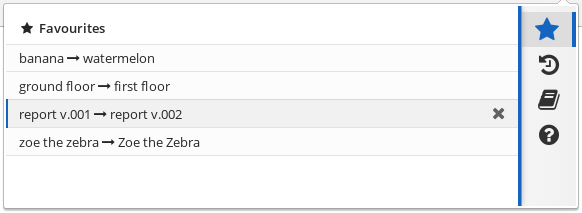
\includegraphics[width=0.99\textwidth]{../main/images/help/fav-step-3.png}
\caption{Favorites Panel Tab}
\end{figure}

\section{History Panel}
The history panel has a similar user interface and functionality as the favorites panel, but instead of leaving the decision to store the given search state up to the user, we add items automatically. We also make sure that we only add meaningful items that resulted in a successful search and replace operation, rather than storing every single change of the search UI.

\begin{figure}[h]
\centering
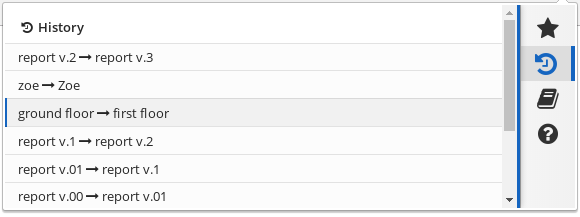
\includegraphics[width=0.99\textwidth]{../main/images/help/history.png}
\caption{History Panel Tab}
\end{figure}

\section{Templates Panel}
Templates allow users to define a piece of text which can later be pasted into the active input area. This could be a signature, a commonly used email response, or any other piece of text that the user is planning to reuse often.

\begin{figure}[h]
\centering
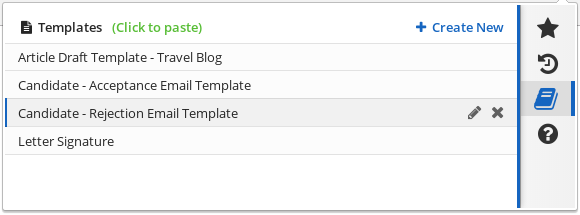
\includegraphics[width=0.99\textwidth]{../main/images/help/templates.png}
\caption{Templates Panel Tab}
\end{figure}

Later we also implemented text transformation commands that appear in this tab whenever there is an active text selection present in the page. This allows users to transform a piece of text to either lower case or upper case with a single click. This is useful because changing text case is in general not an operation easily performed by using regular expressions.

The operations that can be performed using the templates panel are designed for more advanced users, and that is why we decided to move this functionality to this separate panel, rather than trying to include everything in the main search UI.

\section{Help Panel}
The help panel contains links to the official website, feedback forms, as well as a link to the official help text. It also allows users to read through the privacy policy. Since all the data collected is based around usage statistics via Google Analytics, we were able to use a third-party tool \textit{iubenda} \cite{A25} to have the privacy policy text generated for us.

At the same time, this tab gives users an option to opt-out of all Google Analytics reporting via a simple switch button. This was an important privacy requirement that had to be implemented.

\begin{figure}[h]
\centering
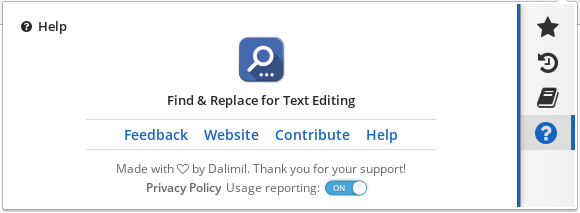
\includegraphics[width=0.99\textwidth]{../main/images/help/help-panel.png}
\caption{Help Panel Tab}
\end{figure}

We also designed a user help guide that explains how to use the extension covering everything from the very basic search functionality all the way to the most advanced use cases (see figure for preview). We open this help text in a new tab right after the extension is installed.

\begin{figure}[h]
\centering
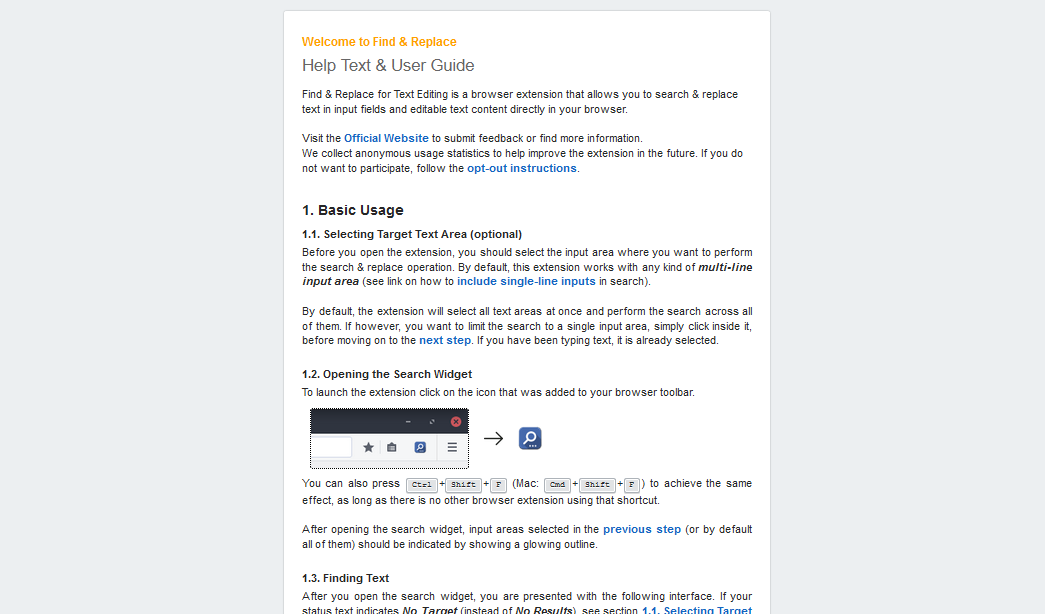
\includegraphics[width=0.99\textwidth]{../docs/help-text-screenshot.png}
\caption{User Guide Page Preview}
\end{figure}

\section{Testing}
The Chrome Extension Developer Guides contain a section on debugging \cite{C3} but any standardized extension testing approaches are nonexistent. Due to technology similarities, we can examine how we could test our extension if it was a standard web application.

In such case, we would have several kinds of tests (see \cite{A11}): unit tests testing individual functions, integration tests testing several modules working together, and functional tests testing scenarios using the whole product (in-browser interaction in our case).

\subsection{Unit Tests}
Our content script contains a lot of individual functions that we can test separately. We used \textit{Mocha.js} \cite{A12} for unit testing of individual methods in the content script and search widget. The coverage will be very limited however, because most functions need to interact with the \textit{Document} and \textit{Window} objects, which are supplied by the web browser and will be undefined when running a command line test. We therefore shift our main focus to integration tests and functional tests.

\subsection{Integration Tests}
We would like to test if multiple modules or parts of our code can work well together. We split this into tests for the search widget, and tests for the content script. Testing the extension working as a whole will be addressed in the Functional Tests section.

\subsubsection{Search Widget Tests}
Our UI search widget is mostly focusing on keeping the state of the UI consistent. Here we are more interested in the widget being rendered correctly as a whole, and that the UI doesn't accidentally change in unexpected ways.

Because of the way we separated the search widget development (described earlier), we could simply mount our React root on a standard website's DOM node and test basic user interaction. There will be no content script for it to communicate with, but this is not the focus at this point.

Because the search widget code is written using React, we used React's testing tool called Jest, which makes it very easy to test React components (see Jest Snapshot Testing \cite{A13}). It is using a specifically designed test-renderer that instead of spinning up an actual browser instance to render a visual component, it creates a snapshot of the resulting HTML and writes it into a file. These snapshots are regenerated on subsequent test runs and compared to the old versions. That way it can quickly discover and report any changes (and mark that particular test as failed in such case).

\subsubsection{Content Script Tests}
What we are interested here is, given a simple website, can the injected functions from our content script work together, so that when triggered by a mocked API call, they successfully perform the find operation and highlight occurrences.

We achieved this by creating a simple HTML page that already includes all the code that the extension normally injects into a web page. In addition to that, we included one more script file that contains the actual test suite.

Unfortunately, the content-script hides its scope in an isolated JavaScript sandbox, so simply including it in a local HTML page will not allow us to interact with it in any way, because the connection API that it uses is only made available to the script when it is injected via an extension.

We therefore needed to detect when the content script is running in the debug mode and not as a part of an installed extension (the state when the runtime connection API is undefined is a good indicator of that) and we exposed the API message handling function when this was the case, which allowed us to mock the API and perform our tests. We recorded a short preview video to show how these content-script tests run in browser (YouTube link): \url{https://www.youtube.com/watch?v=_SzxjBO75mE}

\subsection{Functional Tests}
To implement functional tests, we would need to drive a browser that installs our extension and interacts with it. There is a tool called PhantomJS \cite{A14} which is commonly used for headless WebKit testing. Unfortunately, it is not based on Chromium, so we cannot load Chrome extensions.\footnote{\url{https://stackoverflow.com/a/23643111}}

To be able to install and test the extension as a whole in Chrome and Firefox, we used Selenium \cite{A15}, which is a browser automation tool that can directly control a browser instance and allows us to install browser extensions as a part of the testing process.\footnote{\url{https://stackoverflow.com/questions/15005833/browser-plugin-testing-with-selenium/17117849}}

We installed Selenium WebDriver to control Chrome and Firefox browsers. The Selenium WebDriver accepts commands via a client API and sends them to the browser (see \cite{W2}). The client API has several implementations in various programming languages. We decided to use JavaScript to keep the whole code-base consistent. 

The Selenium project have their own JavaScript implementation for the client API, but after comparing it to alternatives, we decided to use WebDriverIO \cite{A16} instead, which is another JavaScript implementation of the (Selenium 2.0) WebDriver API, but it has much simpler and more readable syntax.

\subsubsection{Browser Automation Tests}
We created a test that checks that after the WebDriver spins up a new browser instance (Chrome or Firefox) and installs our extension, a new tab is created with our help text (user guide), which is the default behavior our extension should follow immediately after being installed.

Unfortunately the WebDriver does not allow direct mouse interactions with the extension -- there is no way to launch it from the toolbar (mentioned in \cite{A17} and \cite{A18}). At the same time, we designed the extension with the minimal set of permission needed, so the extension does not execute any code or inject anything into the web page unless the user launches the extension widget first.

The only way we could overcome this limitation would be to create a new extension that forces the injection of the content script code in every page the browser visits and also automatically starts sending the exact data payloads mocking the API calls coming from the (never running) search widget. Besides it being loads of work to implement, this would not actually be the full functional tests that we were aiming for -- it would be testing the content script alone but none of the actual component interaction and communication with the search widget. We abandoned this idea, because we already have integration test for testing the content script functionality alone, so this approach would not increase our test coverage.

\subsection{Manual Tests}
Due to some of the limitations mentioned above and also to speed up initial development of the core functionality, at the early start of the development process a demo HTML page was created. This HTML page contains all possible combinations of editable text areas -- all types (plain textarea, contenteditable, and single-line inputs), all sorts of styling, various states such as with a scrollbar, or in a scrollable container, as well as text areas inside nested iframes, and various other combinations.

It is very quick to open this HTML page in a browser and use the already installed extension to see if everything is working as expected. It also allows for efficient debugging, and troubleshooting a specific element category when things don't work.

Besides using it to manually test that the overall product works, it was also a good test of the overall user experience, as the HTML page contained the various editable elements that users would normally encounter on the web.

\section{Google Analytics}
In order to collect statistics on how users use our extension and how they interact with different UI elements, we implemented Google Analytics into our extension.

Collecting this data requires us to inform users of the data collection and provide a way for the users to opt-out from collecting these analytics. This might dissuade a small percentage of potential users from installing the extension in the first place, but the belief was that this percentage would me small, which turned out to be true.

\subsection{Google Analytics Implementation}
The standard way of implementing Google Analytics is by inserting a short script into a web page, which then pulls more JavaScript code from Analytics servers, to collect user data, as well provide a developer interface to send additional tracking events.

This method does not work in Mozilla Firefox extensions due to their review policies (quoting from \cite{A20}): \textit{...The most popular way to do this is to inject the Google Analytics script into your codebase as if it were a web page. However, this is incompatible with our review policies. Injecting remote scripts into privileged code – or even content – is very dangerous and it’s not allowed.}

As a workaround, we need to use Google Analytics' Measurement Protocol \cite{A21}, which is a simple API that accepts HTTP requests with Analytics data. It collects data (and aggregates it for displaying dashboards and statistics via the same Analytics web interface) without relying on the Google Analytics JavaScript library running on the client, so we essentially had to implement the library ourselves and only send requests in the appropriate format to this API.

\chapter{Evaluation}
\label{chapter:evaluation}

\section{Distribution and Marketing}
The extension was released on Chrome\footnote{\url{https://chrome.google.com/webstore/detail/find-replace-for-text-edi/jajhdmnpiocpbpnlpejbgmpijgmoknnl}} and Firefox\footnote{\url{https://addons.mozilla.org/en-GB/firefox/addon/find-replace-for-text-editing/}} web stores, which is the official place where users can download browser extension. It was then shared on HackerNews, Quora, Facebook, and several subreddits on Reddit.

These sources constituted only a minority of the overall web store visits however, and the major acquisition source remained to be organic Google Search (people who specifically search for this extension on Google rather than learning about it via social media or forum posts). Almost 80\% of all downloads of the extension in the Chrome Web Store are users who came there from Google Search results.

\begin{figure}[h]
\centering
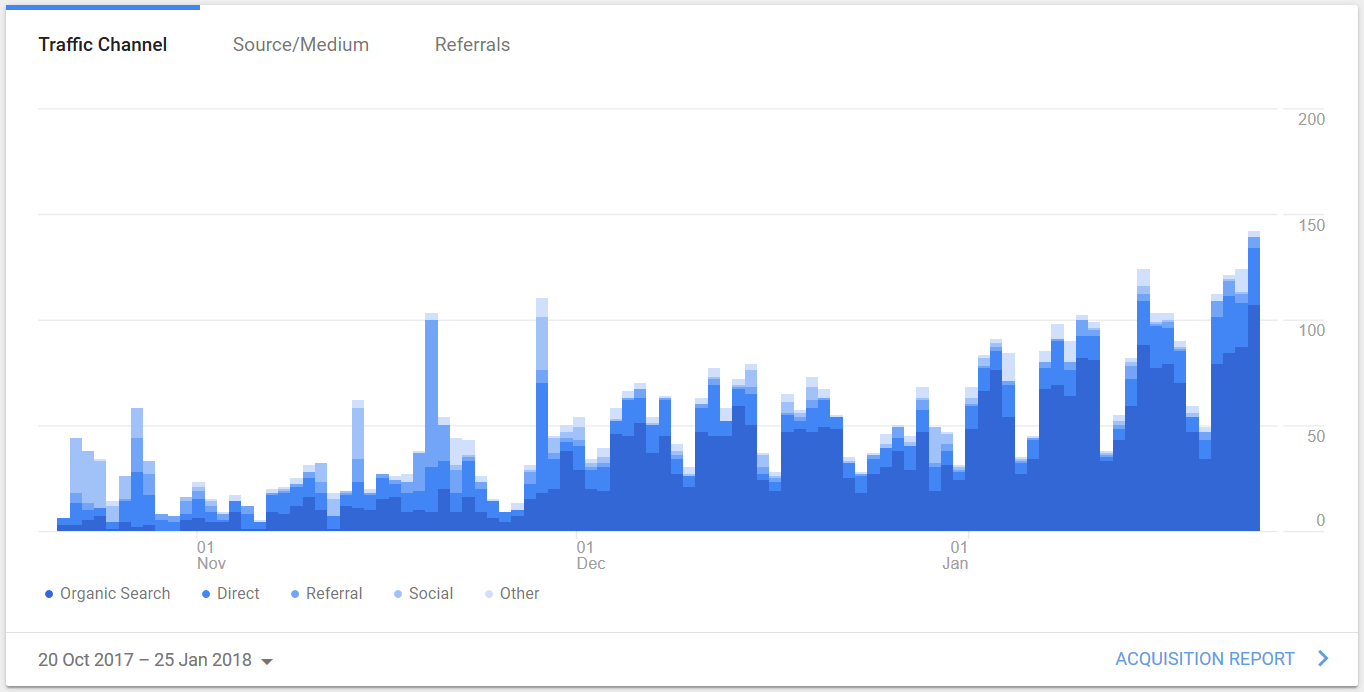
\includegraphics[width=0.99\textwidth]{../docs/user-acquisition.png}
\caption{Chrome web store page -- user traffic}
\end{figure}

The figure above clearly shows a few initial attempts to market the extension on social media and the users who came to the web store page from social links. After that, the graph follows a more regular pattern where the organic Google Search distinctly dominates.

\begin{figure}[h]
\centering
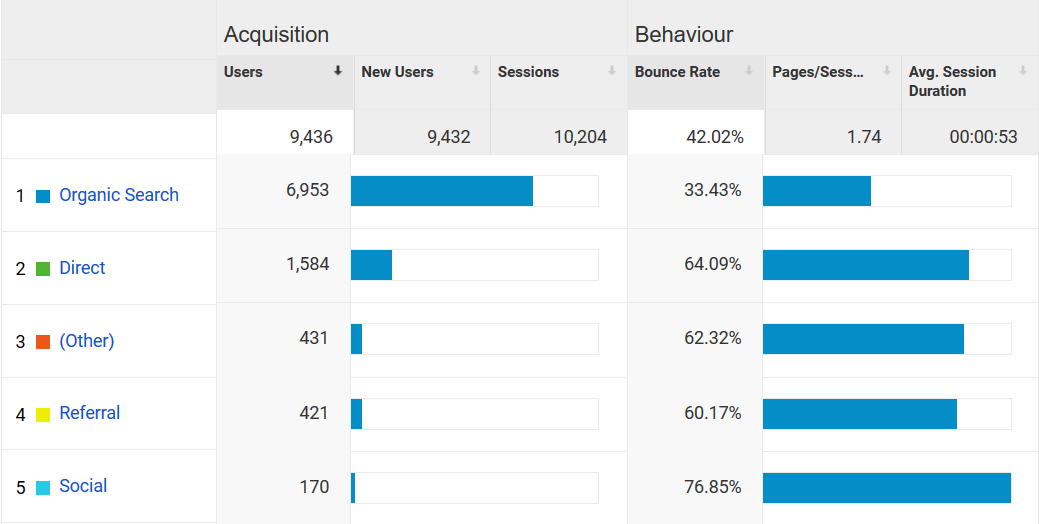
\includegraphics[width=0.99\textwidth]{../docs/user-acquisition-sources.png}
\caption{Chrome web store page -- acquisition sources}
\end{figure}

Since Chrome Web Store allows us to measure Analytics for our web store listing page, we were able to analyze all our main user acquisition sources and obtain the shown graphs. Besides revealing that the most visitors are coming from Google Search results it also showed that these visitors are more likely to install the extension and less likely to immediately leave the web store page (Bounce Rate statistics).

\subsubsection*{Users of Older Extensions}
We also looked at Google users who left negative reviews on the web store for some of the older extensions that tried to implement search \& replace. The users are linked to the reviews only via their (automatically created) Google+ profiles rather than Gmail addresses. Since the Google+ ids are linked to Google Hangouts ids, we managed to send chat invitations to these users, informing them that a new and working search \& replace extension has been released and encouraged them to give it a try. This resulted in numerous five star reviews and overall very positive feedback.

\section{Google Analytics}
We embedded the Google Analytics code into our extension's widget, so that we can track how many times users open the search widget, as well as how many unique users we have, and what kind of population they represent (along with additional user details).

\subsection{Page View Tracking}
Our search widget is essentially a single page application, but we would like to track how many times users open different widget tabs (history, templates, etc.). Therefore we send a `pageview` event every time a user opens a tab, and set the pageview path to the name of the tab. That way we could look at opening tabs as an actual page navigation (inspiration to follow this approach taken from \cite{A22}).

\subsection{Event Tracking}
In addition to the basic user and page view tracking we wanted to know how users interact with our extension and in particular, if they use certain functionality significantly less or more. This might suggest potential ways we can improve our extension - for instance, if nobody ever uses the templates panel, perhaps we need to educate users on how to use it more effectively, or perhaps reconsider its overall usability.

We decided to start collecting the following types of events:
\begin{itemize}
\tightlist
\item
  \textit{Analytics enabled/disabled clicked} -- If the user has allowed Analytics to be used for a week and then opts-out, we want to know they did it (rather than thinking they stopped using the extension)
\item
  \textit{Added to/Removed from Favourites} -- We can get more insight by looking at how often users use the star button. If they have never used it, perhaps it is not intuitive enough.
\item
  \textit{New Template Created} -- Enables us to see how often users create new templates. If the numbers are very low, perhaps they do not know how to use this feature.
\item
  \textit{Template Successfully Pasted} -- Enables us to see how many users have successfully inserted a template into a web page and thus how many know how to use them.
\item
  \textit{Advanced Search enabled/disabled} -- We would like to know how often users use the advanced search functionality (regex search and in-selection search)
\end{itemize}

In the Google Analytics Dashboard we can plot how many of the total number of users triggered that given event in a given time period (see figure).

\begin{figure}[h]
\centering
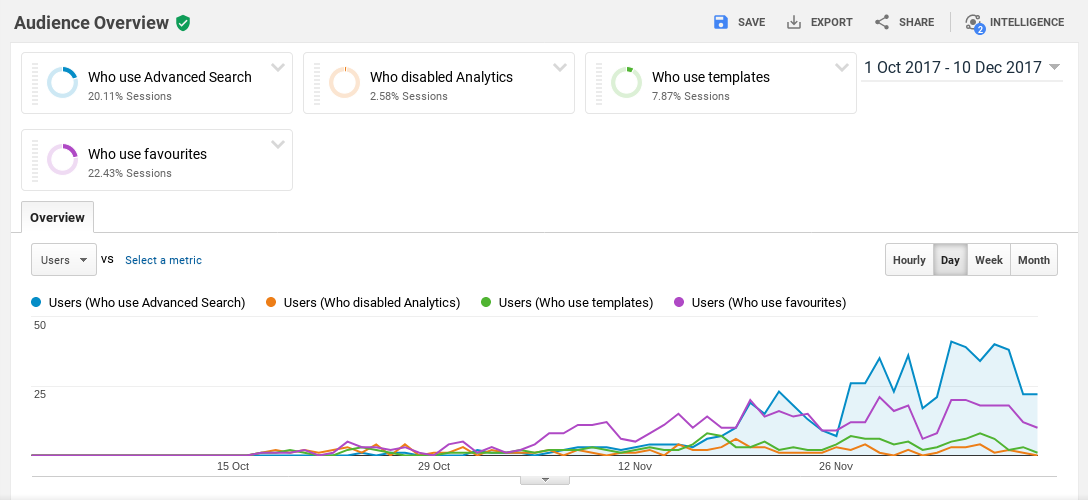
\includegraphics[width=1\textwidth]{../docs/user-behavior.png}
\caption{User behavior and feature usage}
\end{figure}

We can clearly see that a large portion of people use advanced search and the favorites panel. However, only a small portion use templates. This corresponds to the data that we obtained from tracking the page views (tab views), where a lot of people access the favorites and history tabs, but only a few visit the templates and help tabs.

\subsection{Domain Tracking}
A lot of the feedback messages that were submitted after someone uninstalled the extension were not very useful and often looked something like \textit{not working}. This is not very helpful as it does not tell us on which sites they tried to run it that didn't work for them. The analytics that we have been collecting gave us insight into which features of the extension were more used than others but told us nothing about the sites where the extension was actually used.

To get a better idea of which sites are the most frequently used and which should therefore receive more attention (to make sure everything works as expected), we decided to anonymously collect domain names (not URLs, only host names, for privacy issues). This allowed us to construct a list of the top domain names where the extension is used most frequently. We therefore added a Google Analytics event that reports the domain name whenever the extension is used. We then combined unique events from each user to create the list.

\begin{figure}[h]
\centering
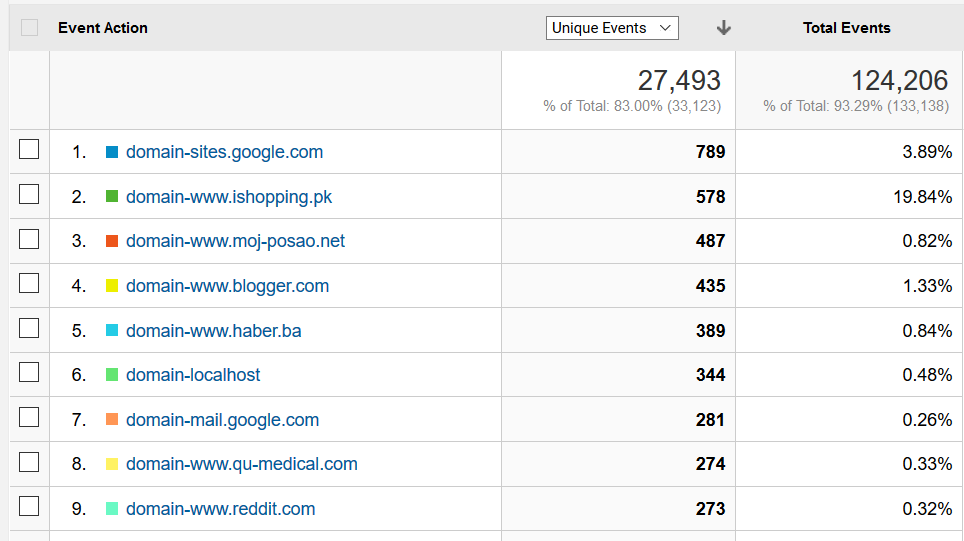
\includegraphics[width=1\textwidth]{../docs/top-domains.png}
\caption{Top domains after 2 weeks of reports. 13th January 2018}
\end{figure}

We used this list to better understand our users. For instance, it led to discovery of people who were trying to use the extension in Google Docs, and also on localhost for Jupyter Notebook. These two specific domains and their handling in code is discussed in later chapters.

\section{Support Website}
There are various ways we could collect user-submitted feedback. We could have a website that provides a contact email address or asks users for a feedback message and sends the email automatically. This email inbox could get very cluttered and hard to manage, especially since we want to collect various forms of feedback (e.g. did the user recently uninstall the extension, or are they happy and simply want to propose new features?). 

We decided to proceed with an alternative solution of creating a support website and storing all submitted feedback messages in a database. This database can later be queried and filtered based on various criteria (time of submission, feedback type -- general feedback vs complaint after uninstalling, ...), which simplified feedback evaluation.

We created a static landing page website that presents the extension with relevant links to the browser web stores, and also allows users to submit feedback via a simple form.

\begin{figure}[h]
\centering
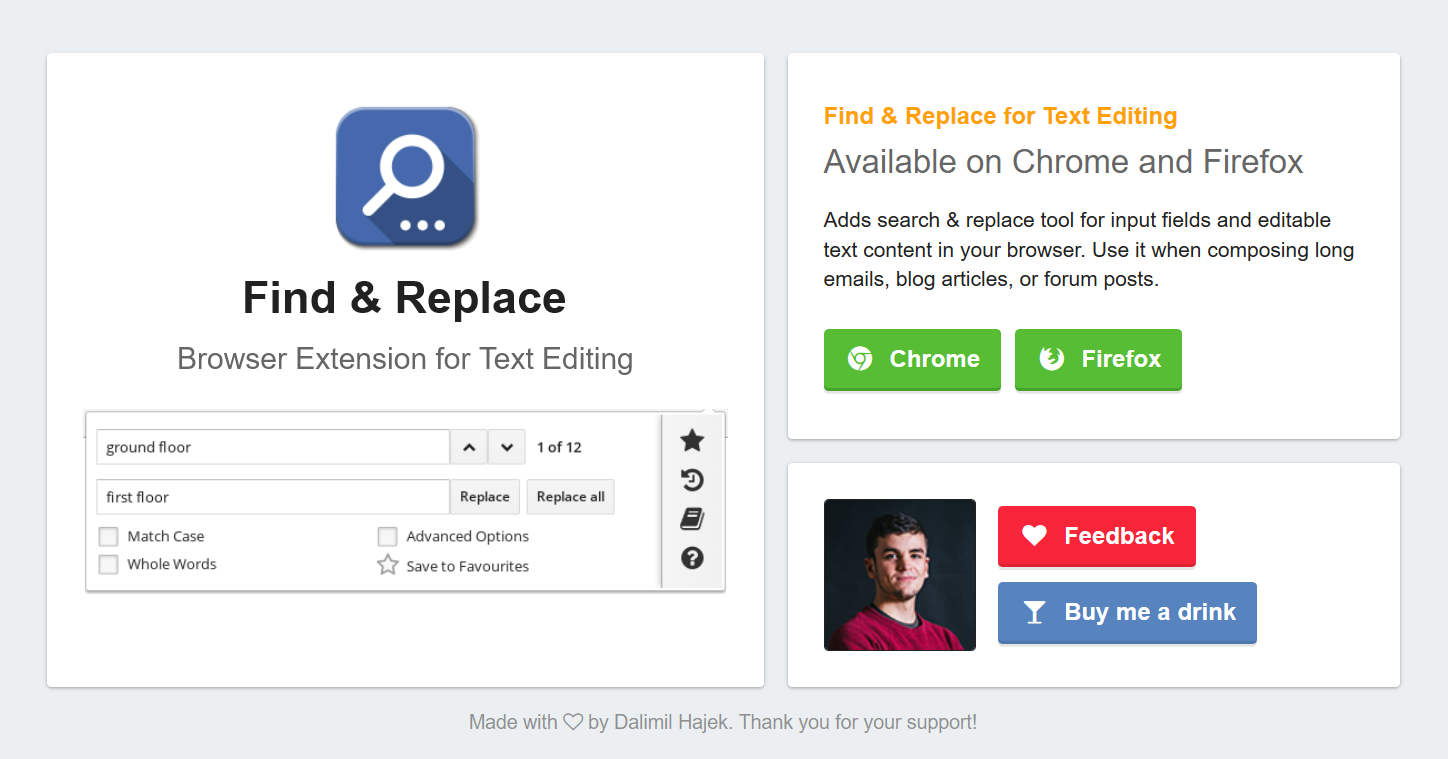
\includegraphics[width=0.99\textwidth]{../graphics/landing-page.png}
\caption{Support website landing page}
\end{figure}

The website was deployed using Firebase Hosting \cite{A8}, which is Google's hosting for deploying static content to its content-delivery network (CDN).

The database used to store the feedback comments is Firebase Realtime Database \cite{A9}, which is a NoSQL cloud database from the same family of Google products. This allowed us to have a secure place to store our data with minimal setup time. It also allowed us to have an optimized static website with only the required JavaScript SDKs without having to implement a complex back-end server.

At the time of writing, we have received 274 uninstall feedback comments (submitted via a form that appears when users uninstall the extension) and 17 general feedback comments (feedback that active users leave after clicking on the feedback link in the extension Help tab or alternatively directly via the website).

\section{Iteration}
After the initial web store release we continued to collect feedback from users, and subsequently kept releasing updates to the extension that were fixing bugs and issues that we found, or were adding features to the extension. The full changelog for specific releases can be found below.

About eight releases were a direct response to written user feedback that I received, submitted either via feedback forms or (in about five cases) via a direct email message. Further, about six releases were linked to discussions with the project supervisor, about two were a reaction to data received through Google Analytics, two were addressing the results of our user study, and the rest of the releases were results of own ideation or simply work that had to be done on the extension.

\paragraph*{Changelog}
\begin{itemize}
\tightlist
\item
\texttt{v1.3.15} -- 12th Mar -- Fix newline pattern in regex replace
\item
\texttt{v1.3.14} -- 26th Feb -- Add undo action for text-case transform
\item
\texttt{v1.3.13} -- 26th Feb -- Fix text-transform templates usability
\item
\texttt{v1.3.12} -- 3rd Feb -- Implement auto-save in templates panel
\item
\texttt{v1.3.11} -- 29th Jan -- Fix Firefox extension chrome object
\item
\texttt{v1.3.10} -- 29th Jan -- Add text case transform templates
\item
\texttt{v1.3.9} -- 14th Jan -- Support local debug mode for testing
\item
\texttt{v1.3.8} -- 14th Jan -- Fix \textit{No Target} indicator
\item
\texttt{v1.3.7} -- 13th Jan -- Add Google Docs warning notification
\item
\texttt{v1.3.6} -- 2nd Jan -- Add support for single-line input fields
\item
\texttt{v1.3.5} -- 31st Dec -- Add hostname to GA for domain analysis
\item
\texttt{v1.3.4} -- 19th Dec -- Fix \textit{Replace all} with regex groups
\item
\texttt{v1.3.3} -- 19th Dec -- Fix restored favorites not storing state
\item
\texttt{v1.3.2} -- 18th Dec -- Fix undefined regexp groups substitution
\item
\texttt{v1.3.1} -- 27th Nov -- Add info notification for broken sites
\item
\texttt{v1.3.0} -- 27th Nov -- Implement dynamic mark tags based on site
\item
\texttt{v1.2.1} -- 18th Nov -- Add more events to GAnalytics
\item
\texttt{v1.2.0} -- 18th Nov -- Change templates to \texttt{execCommand} API
\item
\texttt{v1.1.3} -- 25th Oct -- Fix bugs in replace offsets
\item
\texttt{v1.1.2} -- 23th Oct -- Add help text links
\item
\texttt{v1.1.1} -- 23th Oct -- Add UI hints
\item
\texttt{v1.1} -- 20th Oct -- Disable all debug logs
\item
\texttt{v1.0} -- 18th Oct -- First prototype released
\item
\texttt{v0.1} -- 13th Sep -- Raw dev work started
\end{itemize}

\section{User Study}
To learn how first-time users try to use the extension, we created an online challenge\footnote{\url{https://find-and-replace-f6588.firebaseapp.com/challenge.html}} consisting of five tasks, each involving usage of different parts of the extension functionality. The first two tasks were focusing on the pure search \& replace operation. The remaining were testing additional features in extension's tabs (history, templates, etc.). For instance, to complete the final task one had to transform given paragraph to upper case, save it as a template, and subsequently use the template in their Gmail web app.

Instead of letting people play with the extension on their own (and conducting interviews afterwards), we decided to ask participants to complete our set of tasks and observe their behavior. The extension targets a specific group of people who frequently edit text, so physically meeting a large number of real users in a short period of time would have been problematic. The reasoning behind our challenge was to force participants to work on tasks that real users very frequently tackle, and thus get them into the right mindset when they are testing our extension, no matter their background.

This user session was run with multiple individuals from the School of Informatics at the University of Edinburgh. These users could be described as slightly more advanced as they had working knowledge of regular expressions, yet it was their first time using this extension.

The results after observing the users and talking to them afterwards clearly showed that even though first-time users have no difficulty using the search \& replace user-interface including more advanced functionality, most of them struggled to use the templates panel correctly when they first used it. 

\begin{figure}[h]
\centering
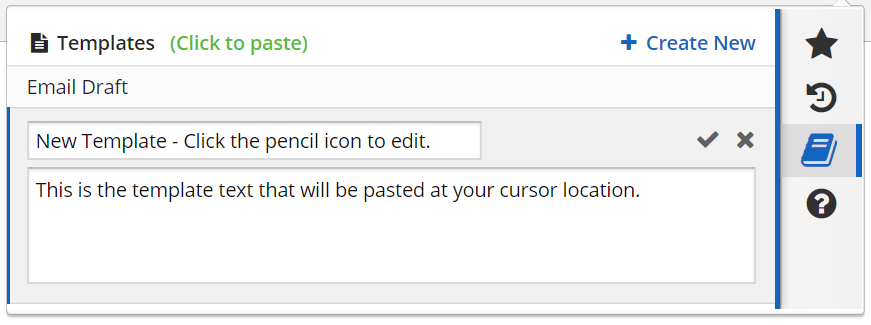
\includegraphics[width=0.9\textwidth]{../docs/template-edit-mode-old.png}
\caption{Template panel -- Old editing mode}
\end{figure}

The issue was that when users starts editing a template, they must click either the \textit{Save} or \textit{Cancel} icon before they exit (see figure). Many people closed the extension by clicking into the page (the browser closes the pop-up widget in such case -- this cannot be overridden), and thus lost their changes.

We have done some research around the topic and (after reading \cite{A26} and \cite{A27} and comparing advantages of several approaches) we decided to implement the auto-save pattern with the saving status indicator similar to the one used in Gmail. The indicator switches between the \textit{Saved} and \textit{Saving...} states as saving to storage takes place in the background. 

This prevented users from losing their template changes, while still allowing them to revert their edits using the \texttt{Ctrl+Z} keyboard shortcut.

\begin{figure}[h]
\centering
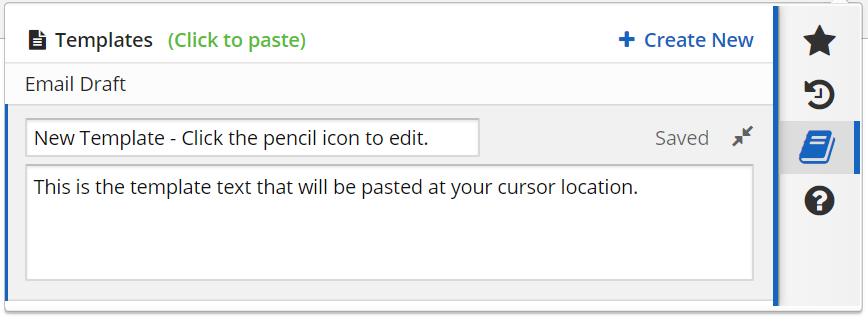
\includegraphics[width=0.9\textwidth]{../docs/template-edit-mode.png}
\caption{Template panel -- New editing mode}
\end{figure}

To make things slightly more efficient we implemented a debounce function \cite{A28} for our template editing mode. This means that instead of attempting to start saving changes immediately we wait a few milliseconds to see if the user is going to continue typing or is taking a break. In the former case, we delay our saving operation. Our implementation turned out to be slightly more challenging since we allow for multiple templates to be edited at the same time, which means we had to make sure we scope each debounce function to the right component.

\chapter{Conclusions}
The extension has received excellent reviews and at the time of writing has over 4000 weekly users (users from both browsers combined), $4.7/5$ stars (19 reviews) on the Chrome Web Store and $4.9/5$ stars (7 reviews) on the Firefox Web Store.

In February it was featured in a Medium article\footnote{\url{https://medium.com/@joisig/startupresources-io-issue-97-36a52e6e8478}} as well as on the \textit{StartupResources.io} page as the Tool of the week.\footnote{\url{http://issues.startupresources.io/archive/93526}}

I have also received a few minor donations via PayPal from users expressing their support for the extension.

\section{Further Work}
Facebook, Quora, and several other sites use contenteditables and keep the text content separately in JavaScript variables. When we insert our highlighting markup, and replace text, their JavaScript immediately restores the previous state (switches back to the original text). We could completely detach their JavaScript listeners, but that stops saving any further changes to the text. This is because the text that is posted is the content of their JavaScript variables, and not the current contenteditable content.

We sought help on StackOverflow, but the only suggestion that received was to try the \texttt{Document.execCommand} API \cite{A10}, which is a mostly deprecated API that was meant to be replaced by contenteditable. It is currently implemented inconsistently across browsers, and using it to replace a piece of text involves manipulating the active cursor selection programmatically. Even after a lot of testing it proved very unreliable and even the W3C specification currently advises against using it.

Google Docs, Jupyter Notebook, or websites using the CodeMirror plugin, are also currently broken. These web apps don't use textareas or contenteditable to store editable text. Instead they implement their own user input handling and then convert, store, and display everything as raw HTML.

Fixing these sites would mean implementing the search \& replace functionality for any source HTML, which is something that we excluded from our scope from the very beginning and instead decided to limit our extension targets to the standard editable text elements.

Google Docs implement their built-in find \& replace tool anyway. When users try to use the extension on one of the above-mentioned websites that are known to be broken, we spawn a small notification informing the user, and cancel the extension's operation.

\section{Final Word}
Overall, bugs and issues that were found were all fixed in subsequent web store releases of the extension. The issues with the sites mentioned above had no straightforward solutions and were either reaching limits of extension API capabilities or were completely out of scope.

In summary, it makes one feel extremely positive, having developed a tool that is used by thousands of people, and which makes their work faster and more productive every day.

% Bibliography section --- use \cite{P1} with BibTeX
\bibliographystyle{plain}
\bibliography{mybibfile}

\end{document}
